\begin{figure}
    \centering
    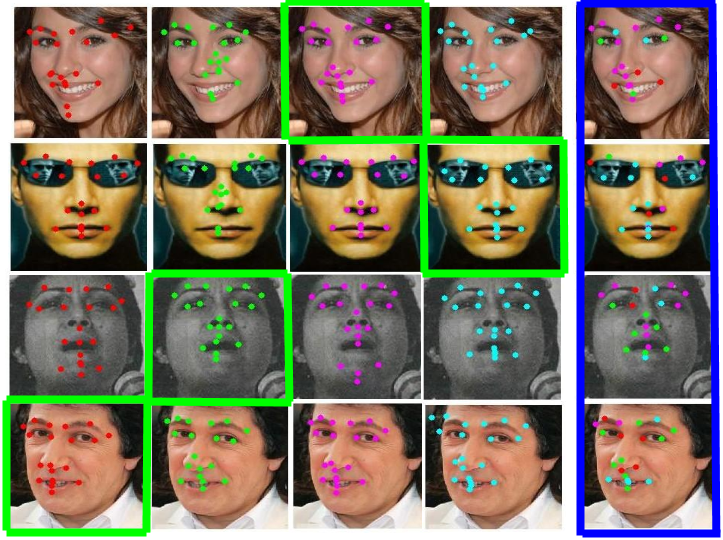
\includegraphics[width=5.5in, height=3.4in]{fid/figures/first_page.png}
    \caption{ Fiducial detection of Chehra [3](red points), Zhu
              et al. [32](green points), Intraface [24](magenta points) and
              RCPR [8](cyan points) can be observed in column 1, 2, 3
              and 4 respectively. Output selection by kNN is highlighted
              in green boxes. Last column shows the output selection by
              optimization highlighted in blue box. Best viewed in color.}
    \label{fig:first_page}
\end{figure}

Facial fiducial detection is an important problem with applications in facial expression 
recognition, gaze identification, face recognition \etc. The task of identifying \emph{several}
locations for different components of a face in an image like ears, nose, mouth \etc., becomes
very daunting considering that each part might have a much more non-distinctive appearance
profile than an entire face, and could also be subject to complete occlusion
(Figure~\ref{fig:first_page}, second row, eyes), drastic appearance and illumination variation
(Figure~\ref{fig:first_page}, third row, pose) or expression variation
(Figure~\ref{fig:first_page}, first row, mouth).
Though there is no consensus
yet on even the number of fiducial points assigned to a face~\cite{smithECCV14_ED}, there is a
broad realization among recent papers for the necessity to reduce failure rates and increase
the accuracy of fiducial detection in a wide variety of challenging examples~\cite{smithECCV14_ED,
zhouICCV13_EGM, koetsingerBFIAT11_AFLW, kumarPAMI13_faceExem,artizzzuICCV13_COFW,yuECCV14_CoR},
since it automatically lends to better performance of systems that rely on fiducial detection.

While a number of different approaches like active shape models~\cite{milborrowCVPR08_ASM},
regression based methods~\cite{yuECCV14_CoR}, cascaded neural
networks~\cite{zhangECCV14_deepfacealign}, tree based methods~\cite{xhuCVPR12_wild} 
and exemplar based approaches~\cite{kumarPAMI13_faceExem}
have been proposed in the recent past, many of these algorithms only
address part of the problems in this area. Since datasets available today like
COFW~\cite{artizzzuICCV13_COFW} ,
LFPW~\cite{kumarPAMI13_faceExem} (Figure~\ref{fig:cofw_lfpw_exemplars}) and AFLW~\cite{koetsingerBFIAT11_AFLW} %(Figure~\ref{fig:cofw_lfpw_exemplars}(b))
offer images varying widely in appearance, pose, expression, illumination and occlusion,
each of these algorithms demonstrate their strengths in specific areas like
occlusion handling~\cite{artizzzuICCV13_COFW}, or robust performance in the
case of profile views~\cite{xhuCVPR12_wild}. Indeed, while regression based approaches are 
better suited to perform well on metrics that measure pixel-wise accuracy
of detection~\cite{milborrowCVPR08_ASM, yuECCV14_CoR}, exemplar or mixture-of-trees based
approaches~\cite{kumarPAMI13_faceExem, xhuCVPR12_wild} are better suited to be
more robust to pose change.


The surprising finding of our work is that many of these algorithms show
decent complementarity in performance, which could be identified and exploited.
% Considering the recent surge in the number of approaches to face fiducial detection,
% and considering their complimentary advantages, it makes sense to attempt a 
% multi-modal approach to fiducial detection. 
In this thesis, we present two algorithms that build on top of recent results in this space. 
Our kNN based algorithm is simple and effective, while our optimization algorithm provides a 
flexible framework to incorporate complicated models. Specifically, our 
algorithms use several state-of-the-art candidate algorithms~\cite{xhuCVPR12_wild, xiongCVPR13_SDM,
artizzzuICCV13_COFW, asthanaCVPR14_Chehra, Tzimiropoulos_2015_CVPR} to generate
fiducial points on a given image, and pose the detection problem as one
of \emph{selecting} the best result from the obtained outputs. By using several
candidate algorithms, we ensure that we have access to the output of different approaches
to fiducial detection, and thus reduce our problem to that of \emph{classifying} 
between accurate and inaccurate fit to the data.

More formally, we propose an \emph{initialization-insensitive}, \emph{pose/occlusion 
and expression-robust} approach to face fiducial detection with the following
characteristics
\begin{itemize}
  \item Our approach attempts the problem of fiducial detection as a \emph{classification}
    problem of differentiating between the best vs the rest among fiducial detection outputs
    of state-of-the-art algorithms. To our knowledge, this is the first time such an approach
    has been attempted.
  \item Since we only focus on selecting from a variety of solution candidates, this allows
    our pre-processing routine to generate outputs corresponding to a variety of face detector
    initialization, thus rendering our algorithm insensitive to initialization unlike
    other approaches.
  \item Combining approaches better geared for sub-pixel accuracy and algorithms designed
    for robustness leads to our approach outperforming state-of-the-art in \emph{both}
    accuracy and robustness.
  %\item We demonstrate the modularity of our approach by modifying an existing 
  %  candidate algorithm~\cite{xhuCVPR12_wild} to use suggestions produce by our approach
  %  to improve detection. We report significant improvements in this case.
\end{itemize}
   
%  \begin{figure*}
%   \centering
%   \subfloat[Input Image]{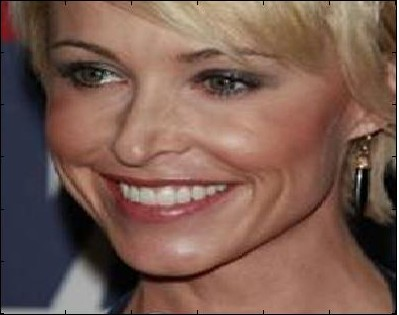
\includegraphics[width=1in,height=0.75in]{fid/figures/im.jpg}}
%   \subfloat[Distance from Exemplars]{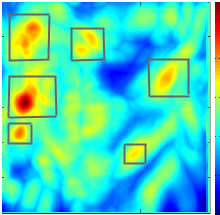
\includegraphics[width=1.5in,height=0.75in]{fid/figures/local_minima_distance.png}\label{fig:distance_map}}
%   \subfloat[Output of Fiducials]{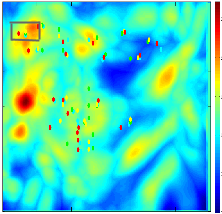
\includegraphics[width=1.5in,height=0.75in]{fid/figures/local_minima_fiducials.png}\label{fig:fid_locations}}
%   \subfloat[Constrained Distance]{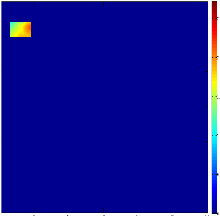
\includegraphics[width=1.5in,height=0.75in]{ffid/igures/local_minima_constrained.png}\label{fig:distance_constrained}}
%   \subfloat[Final Result]{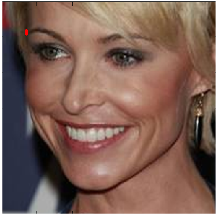
\includegraphics[width=1in,height=0.75in]{fid/figures/local_minima_final_output.png}\label{fig:final_output}}
%   \caption{An example of fiducial detection of eye corner in a test image. Best viewed in color.}
%   \label{fig:example_illustration}
% \end{figure*}

The outline of this chapter is as follows. In section~\ref{sec:related_work}, we review related work
with a perspective to distill out complimentary advantages of different approaches to
fiducial detection. This is followed in section~\ref{sec:face_fiducial_detection} by the 
formulation in section~\ref{subsec:formulation} and outline 
of our approach with focus on exemplar selection (section~\ref{subsec:exemplar_selection}),
output selection (section~\ref{subsec:output_selection} for the kNN algorithm,
section~\ref{subsec:optimization} for the optimization algorithm) and implementation details
(section~\ref{subsec:implementation_details}). We then follow up with an extensive
experimental section~\ref{sec:basic_algorithm}, 
where we first show results on
all the popular datasets like AFLW, COFW, LFPW and in each case
present both mean part-wise pixel accuracy and failure-rate comparisons of our 
approach with the state-of-the-art.
